\documentclass[a4paper,11pt]{article}
\usepackage{tabularx}
\usepackage{graphicx}
\usepackage{wrapfig}
\usepackage{subfigure}
\usepackage{enumerate}
\usepackage{natbib}
\usepackage[center,small]{caption}
\usepackage[top=2cm, bottom=2cm, left=2.5cm, right=2.5cm]{geometry} 

\title{\huge \textbf{Tutorial on using the \textit{spartan} package to analyse agent-based simulation results}\\
\Large For use with \textit{spartan} package version 1.2 onwards
\author{\Large Technique 3: Parameter Sampling and Analysis through use of a \\ \Large Latin-Hypercube approach using SpartanV Interface}
\date{}
}
\begin{document}

\maketitle

\section{Introduction}
\noindent \textit{spartan}, or (\textbf{S}imulation \textbf{P}arameter \textbf{A}nalysis \textbf{R} \textbf{T}oolkit \textbf{A}pplicatio\textbf{N}) is an R package which aids the understanding of the effect aleatory and epistemic uncertainty have on the output from a simulation. This set of tutorials makes use of available example simulation output to demonstrate how a variety of methods can be applied to further understand the results that have been generated.  Following through each example should make it easier to apply the tookit to results generated by any agent-based computer simulation.  This tutorial focuses on the identification of any non-linear effects which occur when two or more parameters are adjusted simultaneously, and uses a java based interface to \textit{spartan} (SpartanV) to perform this analysis.

\section{The \textit{spartan} Package}
\noindent Computer simulations are becoming a popular technique to use in attempts to further our understanding of complex systems. This package provides code for four techniques described in available literature which aid the analysis of simulation results, at both single and multiple timepoints in the simulation run. The first technique addresses aleatory uncertainty in the system caused through inherent stochasticity, and determines the number of replicate runs necessary to generate a representative result. The second examines how robust a simulation is to parameter perturbation, through the use of a one-at-a-time parameter analysis technique. Thirdly, a latin hypercube based sensitivity analysis technique is included which can elucidate non-linear effects between parameters and indicate implications of epistemic uncertainty with reference to the system being modelled. Finally, a further sensitivity analysis technique, the extended Fourier Amplitude Sampling Test (eFAST) has been included to partition the variance in simulation results between input parameters, to determine the parameters which have a significant effect on simulation behaviour.

\section{The Case Study}
\noindent The example simulation results have been taken from an ongoing project which seeks to understand the formation of lymphoid tissue in the small intestine. This simulation outputs cell behaviour measures at various points in the simulation and measures describing the development of the tissue, which occurs through interactions between the cells. Techniques 2-4 of this package allow us to explore how input parameter value affects the behaviour of these cells. We need Technique 1 to tell us how many simulation runs we need for each condition explored to ensure we have a robust representative result.

\section{Scope}
\noindent Do note that the idea of this tutorial is to demonstrate the application of the toolkit, and is not intended to act as a full introduction to using Sensitivity Analysis techniques in the analysis of simulation results. Where useful, links to further reading have been included.

\section{Prerequisites}
\begin{itemize}
\item The R statistical environment, version 2.13.1 or later.
\item The spartan R package, downloaded from the Comprehensive R Archive Network (CRAN) or from the project website.
\item The lhs and gplots R packages, available for download from CRAN.
\item The example simulation data for this tutorial, available from the project website.
\item From version 1.2 of \textit{spartan}, simulation results can be in either CSV or XML format. For earlier versions, results must be pre-processed to be in CSV format.
\item The SpartanV Java Interface for the \textit{spartan} package. Please make sure you follow the installation instructions fully prior to running this tutorial.
\item The Parameter\_Details.csv file available for download from the spartan website.
\end{itemize}

\section{Running Technique 3: Latin-Hypercube Sampling and Analysis}
\noindent Though Technique 2 of this toolkit elucidates the effects of perturbations of one parameter, it cannot show any non-linear effects which occur when two or more are adjusted simultaneously. A Global Sensitivity Analysis technique is needed to identify such effects, and to give an indication of the parameters which have the greatest influence on the simulation output. Thus we have included this method described by Read et al, Saltelli et al, and others (References at the end of this document). A set of parameters of interest are identified, and a range of potential values each parameter could lie within is assigned. A number of parameter value sets are then created through a latin-hypercube sampling approach, which selects values for each parameter from the parameter space, while aiming to reduce any possible correlations when the sample is produced.  A number of simulation runs are then performed for each set generated (this number that which has become apparent through analysis of aleatory uncertainty, or use of Technique 1 within the \textit{spartan} package). The simulation results are then analysed in such a way that any non-linear effects can be identified with ease, both visually and through the calculation of a Partial Rank Correlation Coefficient.  The explanation of this is greatly aided by an example, which is covered later in this tutorial. \\
\\
The \textit{spartan} package includes methods to both create parameter value samples using the latin-hypercube approach, and to analyse the simulation results. This tutorial covers both methods.\\

\section{Parameter Sampling}
\noindent The package contains a method which can produce parameter value sets using Latin-Hypercube sampling. Simulations should then be run on each of the generated parameter sets.  Sampling is performed as follows:\\

\begin{enumerate}
\item Open the SpartanV Java interface to the \textit{spartan} package. Choose Option 4: "Generate Parameter Samples using Latin-Hypercube". Press Next.
\item Now we are going to declare the variables required by the package to produce the parameter value sets. Firstly, use the Directory Browser to select a folder where you wish your parameter value sets to be stored. Then, you need to enter details of each parameter for which you wish to create a range of value samples. You can do this in two ways:
\begin{itemize}
\item Press the "Add Parameter" button and add details on each parameter individually. These details will be name, baseline (calibrated) value, minimum value, and maximum value.
\item Press the "Add Parameter Values From File" button. This is much more useful if you have a large number of parameters. In this tutorial, press this button and find the Parameter\_Details.csv file you have downloaded from the website. Once you have selected this, the parameter details box will populate, as shown in Figure \ref{OAT_Screen1}.
\end{itemize}

\item In box 3, choose the number of samples you wish to take from the parameter space. In this example, we are taking 500 different samples. Then, choose the sampling algorithm that should be used. 'Normal' will randomly sample the parameter space and produce the required number of samples, in a very short amount of time. 'Optimal' seeks to remove any potential correlations in the sampling, and thus is much more computationally expensive and can take a long time (in our experience, 20+ hours for 8 parameters). Choose 'Normal' in this case. Your screen should look similar to that in Figure \ref{LHC_Screen1}. Press Next.

\begin{figure}
\centering
    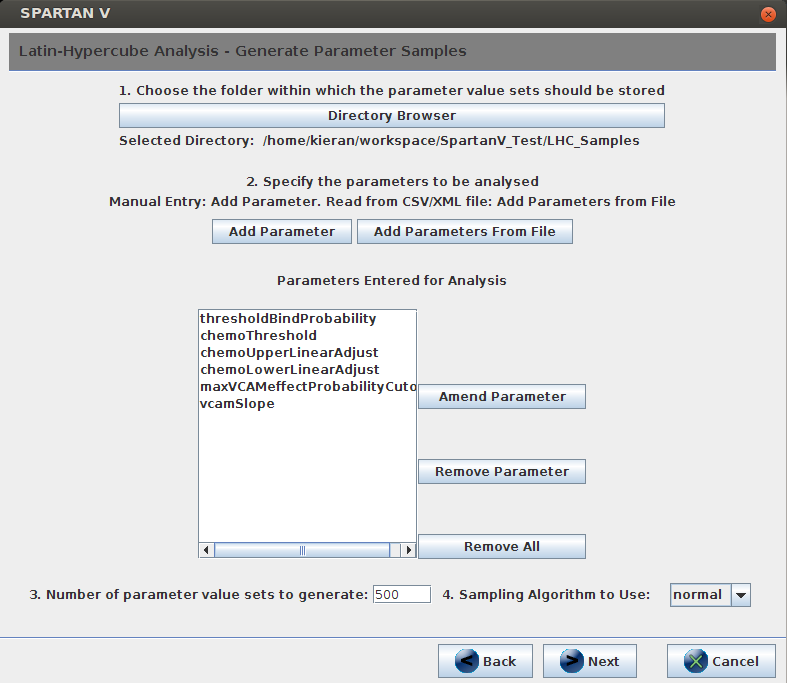
\includegraphics[width=0.8\textwidth]{SpartanV_LHC1.png}\\ \noindent
    \caption{Specifying parameter details for latin-hypercube parameter sampling}
    \label{LHC_Screen1}
    \newpage 
\end{figure}


\item Press the "Generate Parameter Sample Using Latin-Hypercube" button. This will produce a CSV file named LHC\_Parameters\_for\_Runs.csv, containing the required number of parameter space samples, stored in the directory specified in the Directory Browser. Simulations should then be run on each parameter value set in this file, and analysed using the technique in the next part of this tutorial.

\end{enumerate}

\section{Parameter Analysis}
\noindent This section of the tutorial performs this analysis for the lymphoid tissue formation simulation.  In this case, we are going to examine two cell behaviour measures, Velocity and Displacement, that are captured for a period representing one hour of real time, to determine how a change in parameter value influences this behaviour.\\
\\
The assumption is made that for each set of parameters generated by the hypercube, a number of replicate simulation runs have been performed to produce a robust result. This number is elucidated using Technique 1 of this toolkit. So in the example case we are going to use here, we generated 500 different parameter value sets, and for each we have performed 300 simulation runs. The algorithm takes each parameter set generated in turn, processing the simulation results to generate median values for each output measure, for each of the 300 runs. Thus for each of the 500 sets of values, a file is created which shows the median of each output measure for each of the 300 runs. This file can be in either XML or CSV format. A summary file is then created, containing the values of each parameter in that set alongside the median of the 300 medians. An example of such a file can be seen in the data directory of the package (EgSet\_LHC\_Summary.csv). With this summary complete, each parameter being analysed is processed in turn, to determine if there are any correlations between the value of this parameter and simulation output result, although all other parameter values have been perturbed.  Partial Rank Correlation Coefficients (PRCC) are generated for each output measure, for each parameter. These give a statistical indication of any correlations that have now become apparent, and are recorded in a CSV file. An example of this can again be seen in the data directory of the package (EgSet\_LHC\_corCoeffs.csv). To ease identification of such effects, graphs are produced for each parameter, showing the parameter value against the simulation result (output measure).\\
\\
An example will make this clearer.

\begin{enumerate}
\item Download the LHC example data from the project website and extract the results. You will also need the Parameter\_Details.csv file, also available from the project website.
\item The first thing to note is the folder structure.  To use this method, the simulation results do need to be in a specific format (Figure \ref{LHC_Folders} – LHC folder structure).  The structure has two levels:
\begin{enumerate}[(i)]
\item Folders for each set of parameter values being analysed. In the example case, the parameter space was sampled 500 times, thus there are 500 folders, numbered 1-500.
\item A folder for each of the simulation results where the simulation was run under those conditions. Will match the number of runs required that was determined through Aleatory Analysis (Technique 1). So, if this was 300, there would be 300 folders numbered 1-300
\end{enumerate}

\begin{figure}
\centering
    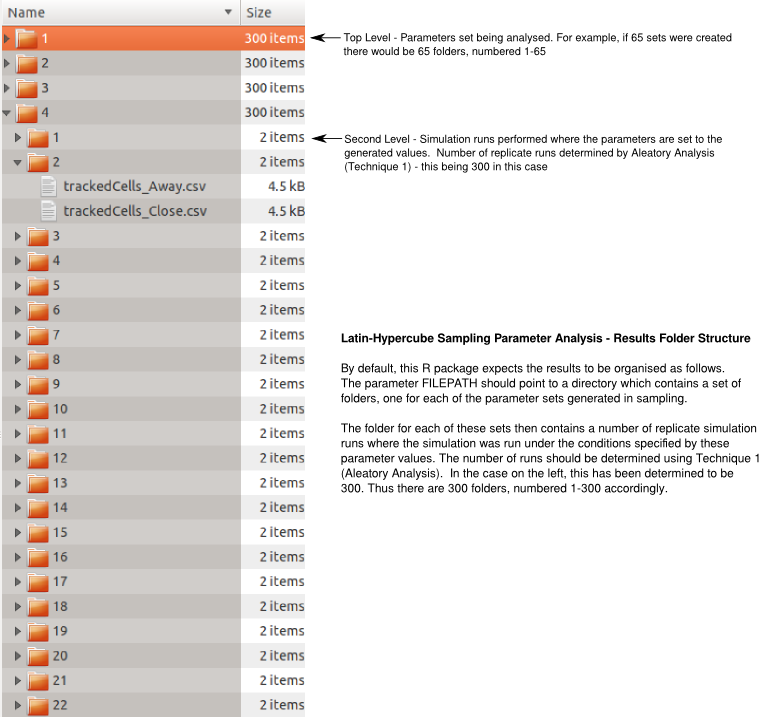
\includegraphics[width=\textwidth]{LHC_Folder_Struc.png}\\ \noindent
    \caption{Simulation results folder structure that should exist for use with this tool}
    \label{LHC_Folders}
    \newpage 
\end{figure}


\item With this data available, open the SpartanV Java interface to \textit{spartan}. Select the fifth method from the choice of analysis methods - "Perform analysis for Latin-Hypercube Generated Samples", and press Next.

\item You will now see the screen in Figure \ref{LHC_Screen2}. Use the Directory Browser to choose the folder that contains the simulation results that you have extracted. Then you will need to enter the details of the two parameters which we are analysing. We will do this by taking the data from the Parameter\_Details.csv file available from the website. This contains the parameters being analysed and the range over which they have been perturbed. This is also available as XML should you prefer that format. So, press the "Add Parameters From File" button and select the Parameter\_Details.csv file. Next, enter the number of samples that were taken from the parameter space (500 in this case), and select the algorithm that was used in sampling ('Normal' in this case). Your screen should look similar to that in Figure \ref{LHC_Screen2}. Press Next.

\begin{figure}
\centering
    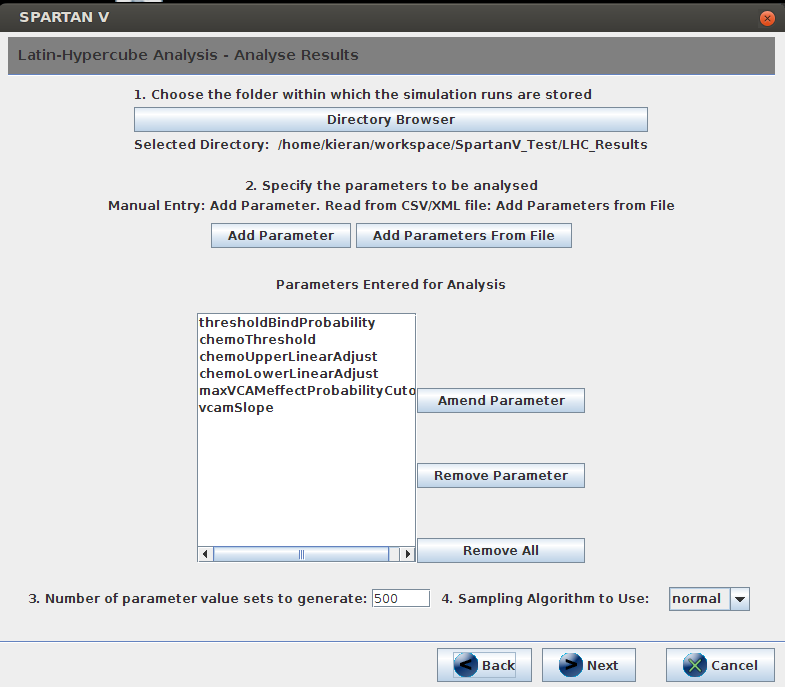
\includegraphics[width=0.8\textwidth]{SpartanV_LHC2.png}\\ \noindent
    \caption{Specifying parameter details for latin-hypercube analysis}
    \label{LHC_Screen2}
    \newpage 
\end{figure}

\item You will now see the screen in Figure \ref{LHC_Screen3}. This screen requests information about the simulator, in terms of output type (\textit{spartan} can process XML or CSV), result file names, and particular columns where the output responses can be found (if csv). For CSV output, it is good to specify result start and end columns to save R errors on duplicate first column entries, and to save reading in whole CSV files. Finally, the screen requests information on simulation timepoints that are being examined. This is covered later in the tutorial. In this scenario, we assume we are only examining one timepoint, and this the last two input boxes are set to NULL. Complete the input boxes with the data shown in Figure \ref{LHC_Screen3} and click Next.

\begin{figure}
\centering
    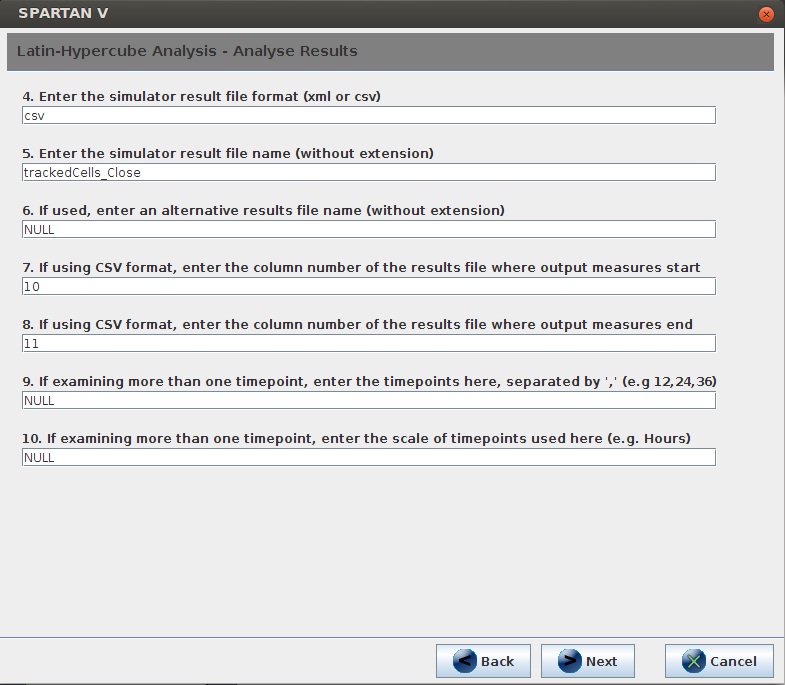
\includegraphics[width=0.8\textwidth]{SpartanV_LHC3.png}\\ \noindent
    \caption{Specifying simulation specifics for this method of analysis}
    \label{LHC_Screen3}
    \newpage 
\end{figure}

\item The next screen (as shown in Figure \ref{LHC_Screen4}) requests information on the simulation output responses that have been examined, the number of replicate runs performed for each parameter value (if this is the case, e.g. for stochastic simulations), and names to assign file names created by the analysis. Firstly however, the algorithm needs to know where the original parameter sampling document (created using the previous technique of this tutorial) has been stored. In the tutorial data, this is in the folder LHC\_Results, and is called Tutorial\_Parameters\_for\_Runs.csv. Use the Directory Browser to select this file. Then complete the remaining data input boxes with the responses in Figure \ref{LHC_Screen4} and press Next.


\begin{figure}
\centering
    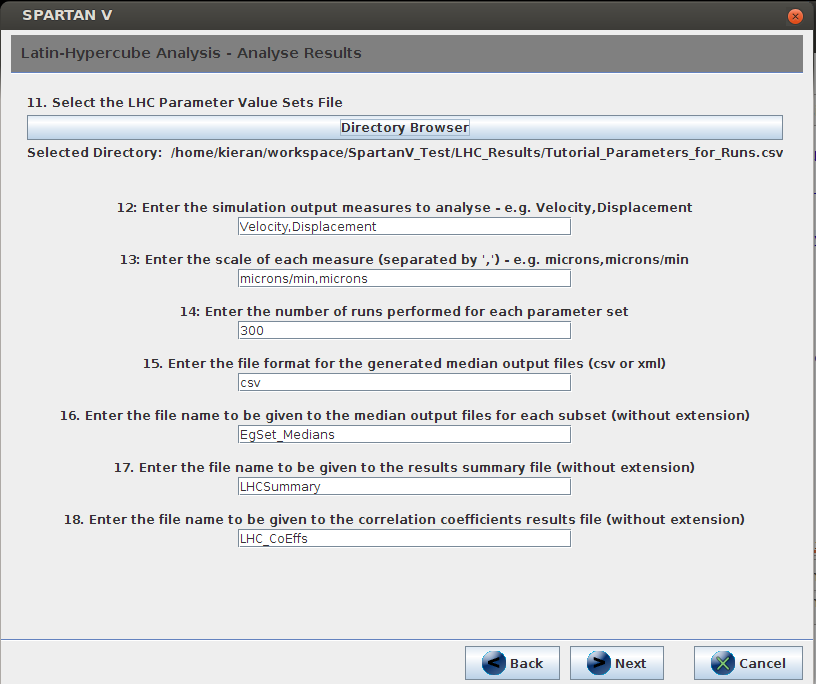
\includegraphics[width=0.8\textwidth]{SpartanV_LHC4.png}\\ \noindent
    \caption{Specifying simulation specifics for this method of analysis}
    \label{LHC_Screen4}
    \newpage 
\end{figure}

\item The final screen asks what methods you wish to run in this analysis. Although you would normally run them all, you may want to run some of these separately, or perform them at different times. These are:

\begin{verbatim}
lhc_process_sample_run_subsets(FILEPATH,NUMSAMPLES,
	NUMRUNSPERSAMPLE,MEASURES,RESULTFILEFORMAT,
	RESULTSFILENAME,ALTERNATIVEFILENAME,OUTPUTCOLSTART,
	OUTPUTCOLEND,MEDIANSFILEFORMAT,MEDIANSFILENAME)
\end{verbatim}

This takes each parameter value set generated by the hypercube in turn, and analyses results from stochastic simulations. Where this is the case, for each parameter set, there should be \textit{n} simulation results. This method goes through these results, producing a file containing the median of each output measure for each of the \textit{n} runs. Thus, if \textit{n}=300, as in our example case, the median file will contain 300 medians for each simulation output measure. The median file generated will be stored with the file name given in MEDIANSFILENAME, in the format specified by MEDIANSFILEFORMAT\\

\begin{verbatim}
lhc_generateLHCSummary(FILEPATH,LHC_PARAM_CSV_LOCATION,
	PARAMETERS,NUMSAMPLES,MEASURES,MEDIANSFILEFORMAT,
	MEDIANSFILENAME,LHCSUMMARYFILENAME)
\end{verbatim}

This again goes through each parameter value set in turn, but this time looks at the medians for each run (stored within the file stated by MEDIANFILENAME). The median of these medians, for each simulation output measure, is calculated. The method then reads in the values that were assigned for each parameter in that run from the sampling result CSV file stated in LHC\_PARAM\_CSV\_LOCATION (a file generated during sampling) and stores the median simulation results alongside the parameter values that were assigned. Once this is completed for all parameter value sets, this is output as a CSV file, filename specified in LHCSUMMARYFILENAME.

\begin{verbatim}
lhc_generatePRCoEffs(FILEPATH,PARAMETERS,MEASURES,
	LHCSUMMARYFILENAME,CORCOEFFSOUTPUTFILE)
\end{verbatim}

Once the summary produced, it is now possible to elucidate any non-linear effects that are apparent when all parameter values are perturbed concurrently. To get a statistical measure of the presence of any effects, the Partial Rank Correlation Coefficient is generated for each parameter. This examines each parameter in turn and each simulation output value, considering the value it has been assigned against the simulation result.  The result of the calculation for each parameter is output to a CSV file, with filename as specified by CORCOEFFSOUTPUTFILE.

\begin{verbatim}
lhc_graphMeasuresForParameterChange(FILEPATH,PARAMETERS,
	MEASURES,MEASURE_SCALE,CORCOEFFSOUTPUTFILE,
	LHCSUMMARYFILENAME,TIMEPOINTS,TIMEPOINTSCALE)
\end{verbatim}

This produces a graph for each parameter of interest, and each simulation output measure for that parameter, plotting the value that parameter was assigned against the simulation result. This makes trends easy to identify. For each graph, the respective Partial Rank Correlation Coeffient is included in the title to give a statistical measure to the results seen visually. 
\\
In normal cases, you would now run all of these methods for a simulation such as that in our case study. However, unlike the tutorials on Technique 1 and 2, actual simulation results have not been included in the download due to the excessive file such from such a large number of simulations runs. Instead, the data included is the output of the first method once run. Have a look at one of the files to ensure you understand the format, but we are not going to run this method, else you will get an error in this case. Instead, untick the checkbox for the first method. Your screen should look similar to that in Figure \ref{LHC_Screen5}. Press Next.

\begin{figure}
\centering
    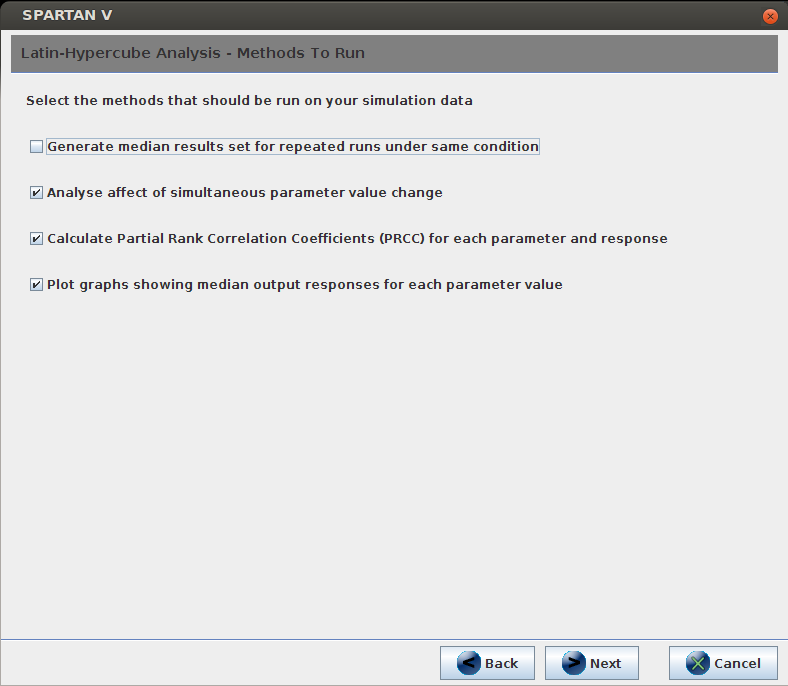
\includegraphics[width=0.8\textwidth]{SpartanV_LHC5.png}\\ \noindent
    \caption{Selection of methods to run in this analysis. In this case untick the first}
    \label{LHC_Screen5}
    \newpage 
\end{figure}

\item On the final screen, press the "Analyse Latin-Hypercube Data" button to start the analysis. The analysis will now run, with updates provided in the console. When the analysis has finished, the following will be produced:
\begin{itemize}
\item Summary of responses under each parameter condition. This will be stored in the LHC\_Results folder, named LHCSummary.csv in this case
\item CSV file containing the Partial Rank Correlation Coefficients calculated for each parameter. This will also be in the LHC\_Results folder, named LHC\_CoEffs.csv in this case.
\item A graph for each simulation response, for each measure, that can be used to determine whether a correlation between parameter value and response has become apparent. Two of the graphs that were generated can be seen in Figures \ref{LHC_Results1} and \ref{LHC_Results2}. Note how for the first parameter, which captures cell adhesion, there is a definite correlation between the Velocity simulation output measure and the value of that parameter, although all other parameters of interest were also being perturbed at the same time.  For the second, which captures the effect of a chemoattractant, note that no such trend has emerged. This gives the suggestion that the value of the first parameter is highly influential in affecting simulation behaviour.
\end{itemize}

\end{enumerate}
\newpage 
\begin{figure}[h!]
\centering
    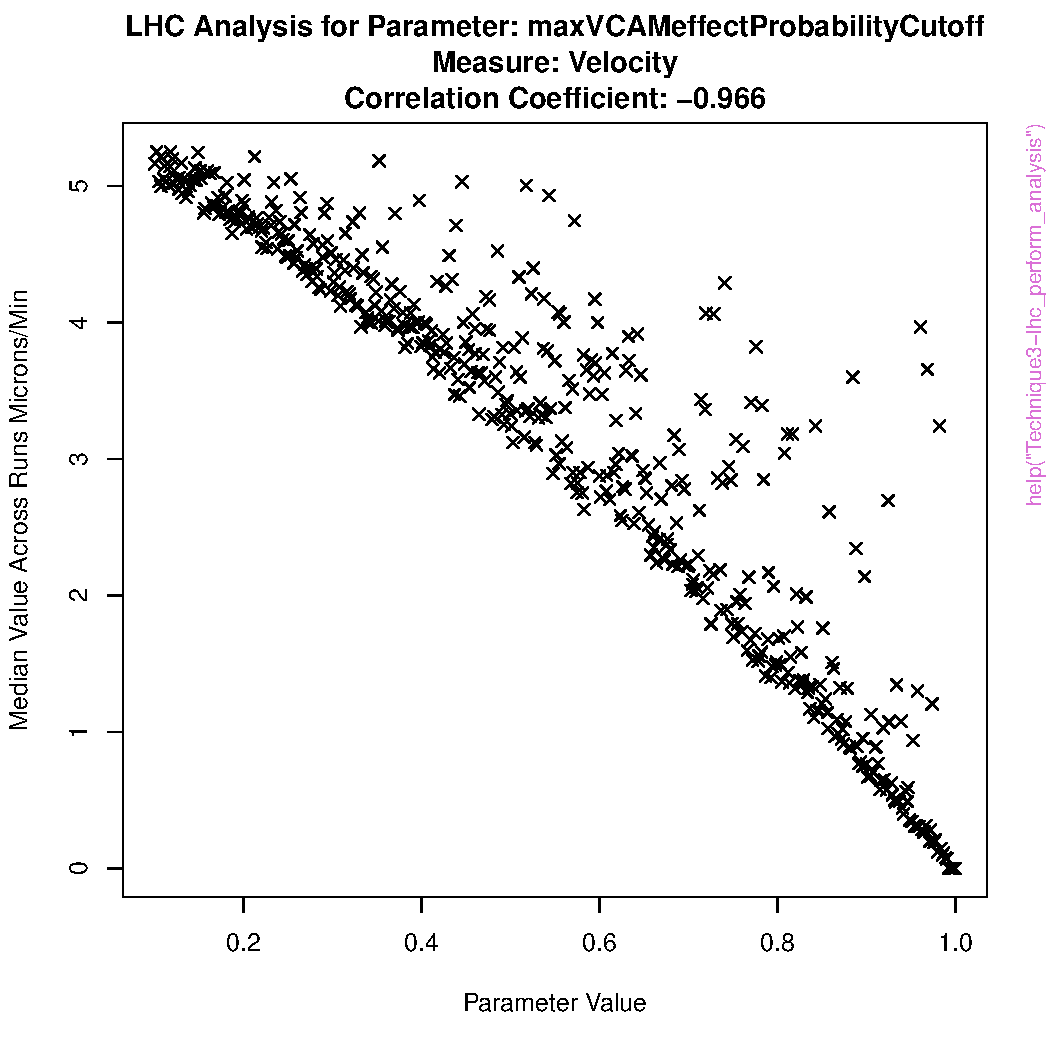
\includegraphics[width=0.65\textwidth]{LHC_maxVCAMeffectProbabilityCutoff_Velocity.pdf}\\ \noindent
    \caption{Graph showing the median velocity observed when the adhesion factor parameter value is perturbed}
    \label{LHC_Results1}
    \end{figure}

\begin{figure}[h!]
\centering
    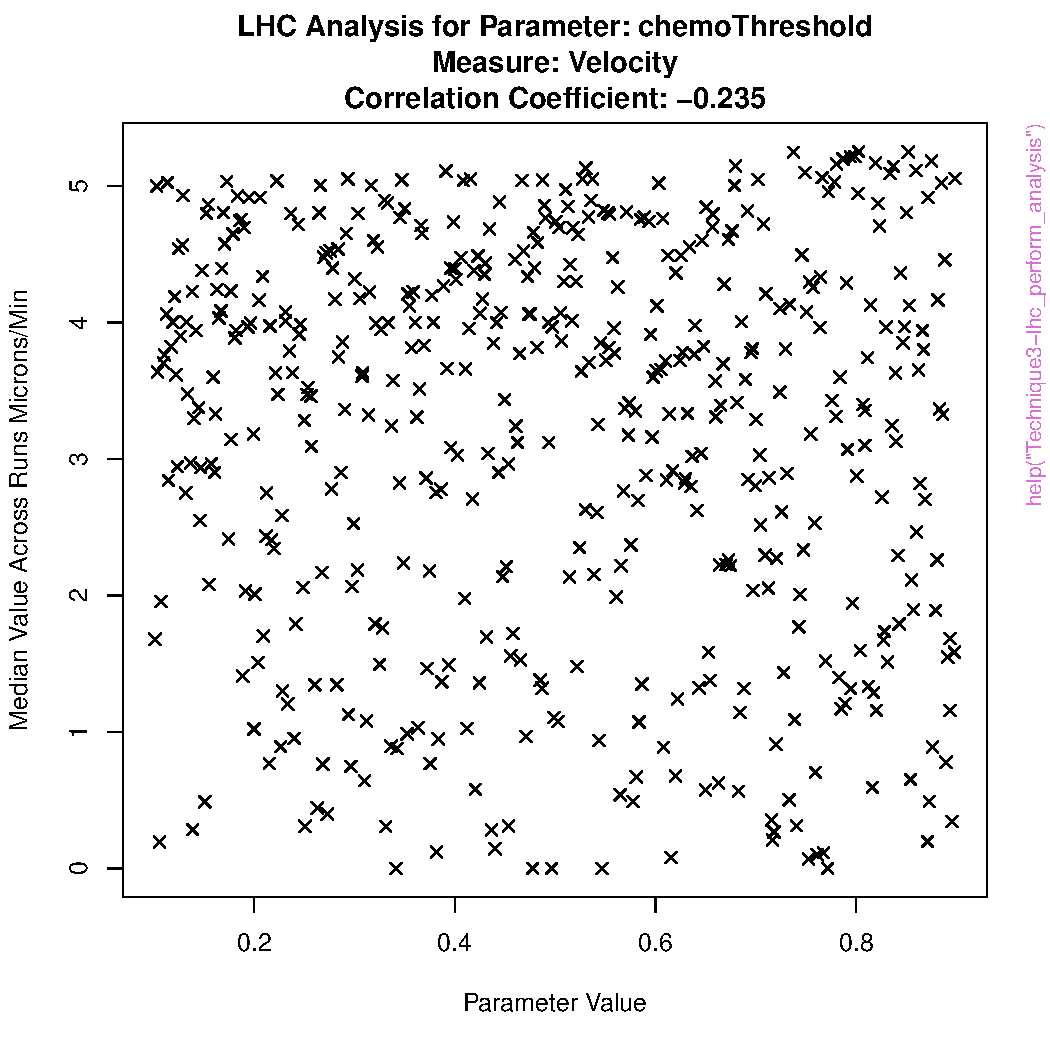
\includegraphics[width=0.65\textwidth]{LHC_chemoThreshold_Velocity.pdf}\\ \noindent
    \caption{Graph showing the median velocity observed when the chemoattractant parameter value is perturbed}
    \label{LHC_Results2}
\end{figure}


\section{Running LHC Technique for Multiple Timepoints}
\noindent The package also has the capability to perform the above analysis for simulation results taken at different timepoints. This may give an indication of when such trends tend to emerge.  Again, we will examine this with an example, yet there is not much to change from the example seen previously\\
\\
In this case study, we have captured the cell behaviour measures at multiple timepoints in the simulation, specifically 12, 36, 48,and 60 hours.  Thus we have the output files trackedCells\_Close\_12.csv, trackedCells\_Close\_36.csv etc. To use this method over multiple timepoints, you should have (a) the same folder structure as in the previous example, and (b) an output file for each timepoint, with the timepoint appended to the filename after an underscore. It is worth writing a script to put your output in this format before looking at this method.\\
\\
Launch the SpartanV interface, and complete Steps 1-4 in the same way as that above. Now, on the second data input screen, enter 12,36,48,60 into box 9 (Timepoints) and type Hours into box 10 (timepoint scale), as seen in Figure \ref{LHC_Screen6}. This tells the analysis that you want to examine simulation responses at four different time-points, with the latter used for graphing results in the final part of the method. Press Next and complete the other data entry screens in the same way. Run the analysis, and statistics will be produced for all four timepoints. 

\begin{figure}
\centering
    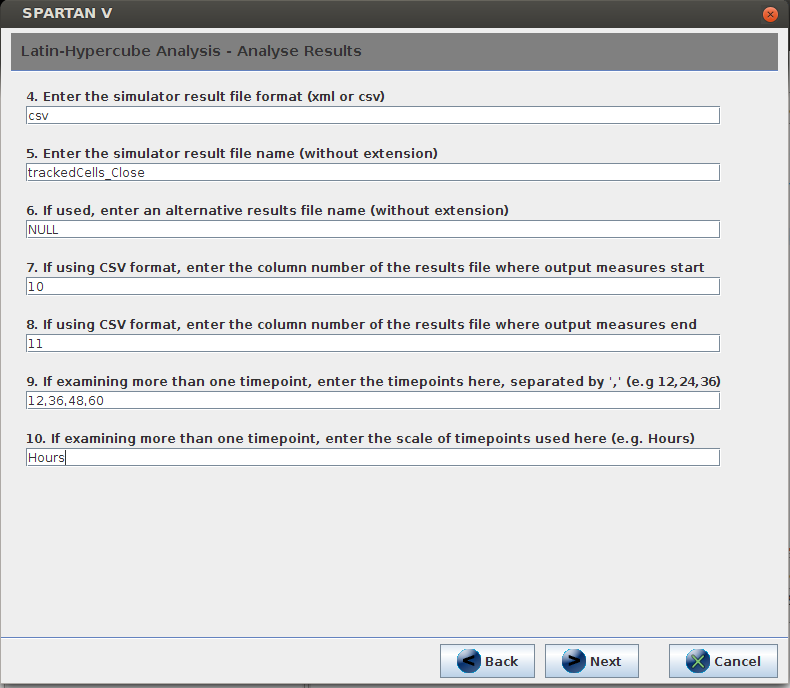
\includegraphics[width=0.8\textwidth]{SpartanV_LHC6.png}\\ \noindent
    \caption{Adding additional time-points to observe effect of parameter perturbation over time}
    \label{LHC_Screen6}
    \newpage 
\end{figure}


\section{Further Reading}
\noindent
The following references may be useful in understanding this technique in more detail:
\begin{itemize}
\item Read, M., Andrews, P.S., Timmis, J. \& Kumar, V. (2012) Techniques for Grounding Agent-Based Simulations in the Real Domain : a case study in Experimental Autoimmune Encephalomyelitis. Mathematical and Computer Modelling of Dynamical Systems, 18(1):67-86.
\item Marino, S., Hogue, I.B., Ray, C.J. \& Kirschner, D.E. (2008) A methodology for performing global uncertainty and sensitivity analysis in systems biology. Journal of theoretical biology, 254 (1), p.pp.178-96.
\item Saltelli, A., Chan, K. \& Scott, E.M. (2000) Sensitivity Analysis, Wiley series in probability and statistics Wiley.
\item The \textit{spartan} Manual, spartan-Manual.pdf, within the spartan package describes in more detail each method within the package
\end{itemize}


\end{document}